\documentclass[11pt, a4paper, onecolumn, twoside,french,cleardoublepage=plain,openany]{report}
\usepackage[english]{babel}
\usepackage[a4paper]{geometry}
\usepackage[utf8]{inputenc}
\usepackage[T1]{fontenc}
\usepackage{indentfirst} % alinea on paragraphs
\usepackage[babel=true]{csquotes}
\usepackage{graphicx}
\usepackage[fleqn]{amsmath} % fleqn = align blocs on the left
\usepackage{siunitx} % SI units
\usepackage{amssymb} % for convolution sign
%\usepackage{moreverb} % for c, cpp snippets
\usepackage[pdfusetitle]{hyperref} % for linkable refs and title in pdf meta

%\usepackage[english,boxed,lined,onelanguage]{algorithm2e}
%\SetAlCapSkip{1em} % Margin between algo and caption
%\SetAlCapNameSty{textit} % text style for  algo captions
\usepackage{algpseudocode,algorithm,algorithmicx}

%\usepackage[toc,page]{appendix}
\usepackage{fancyhdr} % For titlepage \lhead, \rhead... 
%\usepackage[font={it}]{caption}
\usepackage[backend=bibtex]{biblatex}
%\bibliography{bibliographie.bib}
%\usepackage{multirow} % Pour colonnes multiples des tableaux
%\usepackage{longtable} % Pour longs tableaux
%\usepackage{array} % Pour \texttt sur tout une colonne
%\usepackage{xcolor} % Pour éviter que footnote ne bug...
%\usepackage{footnote} % Pour les footnotes dans les tableaux
%\makesavenoteenv{tabular} % Pour les footnotes dans les tableaux
%\usepackage{tabularx}
%\usepackage{pdfpages} % Include des pdfs
%\usepackage[nottoc,numbib]{tocbibind} % Pour faire apparaitre la biblio. dans le sommaire

\usepackage{caption}
\usepackage{subcaption}

\usepackage[]{minitoc} % Intermediate 
\usepackage{etoolbox} % For toggle function (to hide titlepage)
\usepackage[acronym,toc,shortcuts]{glossaries}
\usepackage[english]{cleveref} 
%\makeglossary
%\makeindex

\fancypagestyle{titlepage}{% 
	\lhead{
\includegraphics[width=0.30\textwidth]{logos/logo-enseeiht.png}}
	\rhead{
\includegraphics[width=0.30\textwidth]{logos/logo-imt.jpg}}
	\lfoot{
\includegraphics[width=0.28\textwidth]{logos/logo-univ-ups.png}}
	\rfoot{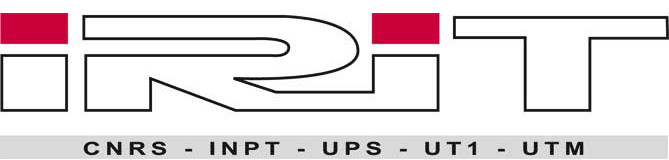
\includegraphics[width=0.28\textwidth]{logos/logo-irit.jpg}}
	\fancyhead[C]{} % On enlève les informations du header
	\fancyfoot[C]{} % On enlève les informations du footer
	\renewcommand{\headrulewidth}{0pt} % On enlève la ligne du header
} \Huge
\fancypagestyle{body}{%
	\restoregeometry 
	\pagestyle{fancy}
	\fancyhf{}
	\fancyhead[LO]{\ifthenelse{\equal{\value{chapter}}{0}}{}{\thesection. \rightmark}} %rightmark = section
	\fancyhead[RE]{\ifthenelse{\equal{\value{chapter}}{0}}
		{}
		{Chapter \thechapter.}
		\leftmark
	} %leftmark = chapter
	\fancyhead[RO]{\thepage} %
	\fancyhead[LE]{\thepage} %
	\renewcommand*{\chaptermark}[1]{\markboth{##1}{}}
	\renewcommand*{\sectionmark}[1]{\markright{##1}{}}
	\renewcommand\headrulewidth{.1pt}
%	\setlength{\parskip}{0.3cm} % Espace entre paragraphes
%	\renewcommand{\arraystretch}{1.5} % Espace entre cases d'un tableau
}
\fancypagestyle{plain}{
	\pagestyle{body}
	\fancyhead[LO]{\rightmark}
}
\fancypagestyle{appendix}{%
	\restoregeometry
	% On nettoie les headers et footers existants de "fancy"
	\fancyhf{}
	% Pour le header
	\fancyhead[RE]{Appendix}
	\fancyhead[LO]{\thechapter. \leftmark} %leftmark = chapter
	\fancyhead[RO]{\thepage} %
	\fancyhead[LE]{\thepage} %
	\renewcommand*{\chaptermark}[1]{\markboth{##1}{}}
	\renewcommand\headrulewidth{.1pt}
	% Pour le footer
	%\fancyfoot[C]{\thepage}
	\renewcommand\footrulewidth{0pt}
}
% \newacronymwithdescr{Label}{Court}{Long}{Description}
\newcommand*{\newacronymwithdescr}[5][]{%
  \newglossaryentry{main-#2}{name={#3},%
  text={(\acs{#2}) #3\glsadd{#2}},%
  description={#5},%
  #1
  }%
  \newacronym{#2}{#3\glsadd{main-#2}}{#4}%
}

% Pas de point final pour les entrées glossaire ou acronymes
\setacronymstyle{sm-short-long}
%\newacronym{IMT}{IMT}{Institut de Mathématiques de Toulouse}
\newacronymwithdescr{IMT}{IMT}{Institut de Mathématiques de Toulouse}{is the main laboratory in mathematics in Toulouse}
\newglossaryentry{Blabla}{name=Blabla,description={is....}}

% To use the glossary entries:
% \acs{} (for short one)
% \ac{} (for long one - only on first appearence)


% MACROS

% Couleurs pour les corrections
\newcommand {\JY}[1] {\textcolor{red}{#1}}
\newcommand {\FR}[1] {\textcolor[rgb]{0.0,0.3,0.0}{#1}}
\newcommand {\OL}[1] {\textcolor{blue}{#1}}
\newcommand {\HW}[1] {\textcolor[rgb]{0.3,0.2,0.0}{#1}}
%\newcommand{\hilite}[1] {\emph{#1}}
\newcommand{\hilite}[1] {\Req{#1}}
\newcommand {\Req}[1] {\textcolor[rgb]{0.75,0.0,0.0}{#1}}
\newcommand {\Geq}[1] {\textcolor[rgb]{0.0,0.5,0.0}{#1}}
\newcommand {\Beq}[1] {\textcolor[rgb]{0.0,0.15,0.60}{#1}}
\newcommand {\black}[1] {\textcolor{black}{#1}}

% Espaces mathématiques
\newcommand {\DPUN} {{\mathcal D}}
\newcommand {\DTREE} {{\mathcal D}^e}
\newcommand {\CC} {\mathbb C}
\newcommand {\RR} {\mathbb R}
\newcommand {\RP} {\mathbb R^{\mathcal P}}
\newcommand {\RPE} {\mathbb R^{\mathcal P \times |\edges |}}
\newcommand {\codeset} {\mathbb R^{\mathcal P \times \leaves}}
\newcommand {\Dset} {\mathbb R^{\mathcal P \times (\mathcal P \#\leaves) }}
\newcommand {\ZZ} {\mathbb Z}
\newcommand {\NN} {\mathbb N}
\newcommand {\PP} {{\mathcal P}}
\newcommand {\HH} {{\mathbb H}}
\newcommand {\II} {{\mathbb I}}
\renewcommand {\SS} {{\mathcal S}} % applis supports
\newcommand {\SA} {{\mathbb S}} % support accessible

% Fonctions
\newcommand {\f}[1] { {\mathcal F}\left( #1 \right) }
\newcommand {\F}[1] { {\mathcal F^{-1}}\left( #1 \right) }
\newcommand {\norm}[2] {\left\| #1 \right\| _{#2}}
\newcommand {\defeq} {\triangleq}

% Opérateurs
\DeclareMathOperator {\sign} {sign}
\DeclareMathOperator {\prox} {prox}
\DeclareMathOperator {\argmin} {argmin}
\DeclareMathOperator {\supp} {supp}
\DeclareMathOperator {\rg} {rg}
\DeclareMathOperator {\diag} {diag}
\newcommand {\RG}[1] {\rg\left( #1 \right)}
\newcommand {\SUPP}[1] {\supp\left( #1 \right)}
\newcommand {\PS}[2] {\langle #1 , #2 \rangle}
\newcommand {\PROBA}[1] {\mathbb P \left( #1 \right)}
\newcommand {\one}[1] {\mathbbm{1}_{ #1 }}
%\newcommand {\one}[1] {\chi_{ #1 }} %{\mathbbm{1}_{ #1 }}
\newcommand {\oneinf}[1] {\chi_{ #1 }}
%\newcommand {\oneinf}[1] {{\mathcal I}_{ #1 }} 

% Acronymes
\newcommand {\PSNR} { \textrm{PSNR}^* } 
\newcommand {\NRE} { \textrm{NRE} }
\newcommand {\CPR} { \textrm{RER} }
\newcommand {\COST} { \textrm{G} } % ancien compression ratio

% Raccourcis
\newtheorem{prop}{Proposition}[section]

\newcommand {\nodes} {\mathcal N}
\newcommand {\edges} {\mathcal E}
\newcommand {\leaves} {\mathcal L}
\newcommand {\NL} {\#\leaves}
\newcommand {\hall} {h^e _{e \in \edges}}
%\newcommand {\multiconv}[1] { \bigstar_{\substack{#1}}\, }
\newcommand {\multiconv}[1] { \mathbf h^{#1}\, }
\newcommand {\tpath}[1] {\mathcal{C}(#1)}
\newcommand {\code} {\mathbf x}
\newcommand {\data} {\mathbf y}
\newcommand {\dataex} {\mathbf b}
\newcommand {\databis} {\mathbf y^e}
\newcommand {\D} {\mathbf D}
\newcommand {\Hs} {\mathbf A}
\newcommand {\Ha} {\mathbf H}
\newcommand {\Haf} {\hat{\mathbf H}}
\newcommand {\Hab} {\bar{\mathbf H}}
\newcommand {\res} {\mathbf r}

\newcommand {\tree}{\mathcal T}
\newcommand{\subtree}[1]{\tree^{#1}}

\newcommand {\stopalgo}{\epsilon}

% autres MACROS
\newcommand {\hkall} {(h^k)_{1 \leq k \leq K}}
\newcommand {\hkconv} {h^1 * \dots * h^K}
\newcommand {\hkconvnorm} {\frac{h^1}{\norm{h^1}{2}} * \dots * \frac{h^K}{\norm{h^K}{2}}}
\newcommand {\hkconvp} {g^{1} * \dots * g{K}}
\newcommand {\hkconvs} {f^{1} * \dots * f^{K}}
\newcommand {\fobj} {\| \code * h^1 * \dots * h^K - \data \|_2^2}
\newcommand {\fobjlambda} {\| \lambda \code * h^1 * \dots * h^K - \data \|_2^2}

% Macros added by Mael
\newcommand{\file}{\texttt}
\newcommand{\dispCode}{\texttt}
\newcommand{\dispCodeLong}[1]{
\begin{verbatim} #1 \end{verbatim}
}
\DeclareMathOperator*{\argmax}{\arg\!\max}% http://tex.stackexchange.com/q/83169/5764

\algnewcommand\algorithmicinput{\textbf{Input:}}
\algnewcommand\Input{\item[\algorithmicinput]}
\algnewcommand\algorithmicoutput{\textbf{Output:}}
\algnewcommand\Output{\item[\algorithmicoutput]}

 % <-- all the \usepackages
\author{Maël Valais}
\date{Updated on \today}
\title{Master's Thesis – Optimization of dictionaries structured in convolutional trees for sparse image representation}
\begin{document}
%\begin{titlepage}
\thispagestyle{pagedegarde}
\newgeometry{tmargin=2.2cm,bmargin=4cm,lmargin=2cm,rmargin=2cm}
\begin{center}
\topskip2.8cm
\textsc{Université Toulouse III — Paul Sabatier}\\
\vspace{0.5 cm}
\line(1,0){100}\\
\vspace{0.6 cm}
{{{Internship Report}}}\\
\vspace{0.3cm}
Defended on September 15\th, 2016\\ \vspace{0.3 cm} par\\ \vspace{0.3 cm} \textbf{Maël \textsc{Valais}}\\
\vfill
{\Huge \textbf{Optimization of dictionaries structured as convolutions trees for sparse image representation }}\\
\vfill

{{Internship at \acs{IMT}}}\\
{Université Paul Sabatier}\\
{118, route de Narbonne}\\
{31400 Toulouse}\\
\vspace{2 cm}

\par Supervised by \\ \textbf{François \textsc{Malgouyres}}\\
Institut de Mathématiques de Toulouse\\ 
%\vspace{1cm}
\par and \\Jean-Yves \textbf{ \textsc{Tourneret}}\\
ENSEIHHT, Toulouse
\end{center}
\end{titlepage}

% Préparation pour les pages de corps
\pagestyle{empty}
\restoregeometry
\cleardoublepage % Blanc jusqu'à prochaîne page paire

\tableofcontents
{\let\clearpage\relax\listoffigures}
{\let\clearpage\relax\listoftables}
{\let\clearpage\relax\listofalgorithms}

\pagestyle{corps} % Uncomment to show title page

\section{Subject and goals}

The current work, mainly developed during Olivier Chabiron's PhD, gives a theoretical frame to the (FTL) problem. The (FTL) problem aims at approximating an ideal dictionary $D^{ideal}$ (which can be easily understood as a matrix) made of ideal atoms $a_i$ on its columns. The approximated dictionary will be called $D$ and the atoms formed by its columns $(H^f)_{f \in \leaves}$. 

But instead of using a standard matrix-vector product to compute $Dx$ and $D^Ty$, the operator $D$ is constituted 
\begin{equation*} \begin{aligned}
Dx
\end{aligned} \end{equation*}

Many image processing techniques are based on... representing the signal ...

We aim... 

Now that it has been proven that the objective function, , actually allows to find local minimums that are close enough to the actual minimum.


The idea behind dictionaries
Say $y$ is a signal we want to ...
We want to find a transform/dictionary D such that, when applied to a code (think of the "transformed" signal) will give an approximated signal $\hat{y}$:

$$D\alpha=\hat{y} \approx y$$

In this work, we will generally stay on the non-noisy case, leaving noisiness to further work.

Algorithm PALMTREE: a Gauss-Seidel algorithm (in the sense that we 

In dictionary learning, we call the columns of $D$ the \emph{atoms}.


This experiment aims to simulate the choice of an atom by the OMP algorithm. As a short reminder, here is the step we are studying:
\begin{algorithm}
    \caption{OMP Algorithm}
  \begin{algorithmic}[1]
    \Require Decomposition of signal $x$
    \Input signal $x \in \mathcal{R}^{m}$, Dictionary $\mathcal{G} \in \mathcal{R}^{m \times n}$, $\hat{x} = \emptyset$
    \Output Decomposed signal $\hat{x}_{\text{est}}$ after $k$ iteration, Residual $R^{(k)}$
    \State \textbf{Initialization} $R^{(0)} = x$
    \While{$i \leq k$}
      \State $l =  \argmax_{l = 1,\dots,l} |\left< g_l,R^{(i)} \right>|$ \label{omp_pick_correlation}
        \Comment{finding the atom in $\mathcal{G}$ with max correlation with residual.}
      \State $R^{(i+1)} = R{(i)}-a_l g_l^{(i)}$
      \State $\hat{x} = \hat{x}+\langle R^{(i)}, g_{l}^{(i)} \rangle g_{l}^{(i)}$
      \State $i = i + 1$
    \EndWhile
  \end{algorithmic}
\end{algorithm}

At \cref{omp_pick_correlation}, the algorithm chooses the column of the dictionary that matches the best the residual. This is where we thought this way of doing would serve our "add an element to one of the supports" algorithm.

% XXX define PALMTREE
Our goal is to, between two iterations of the PALMTREE algorithm, add a new element to one of the supports. That would lead to an optimization-driven construction of the kernels instead of designing them by hand.

But we have been questioning ourselves on the fairness of choosing an element to be added based the mere partial gradient. We remind that the \ref{omp_pick_correlation} is actually computing a gradient:

\begin{align*}
l =& \argmax \left|\left< g_l,R^{(i)} \right>\right| \\
=& \argmax \left| \mathcal{G}^TR^{(i)}\right| \\
=& \argmax \left| \mathcal{G}^T(\mathcal{G}\alpha - u)\right| \\
\end{align*}
So: does the partial gradient \ref{eq_partial_gradient} give 
\begin{align*}
\Phi((h^e)_{e \in \edges}) = \left\| \sum_{f\in\leaves} \code^f * h^{\CC(r,f)} \right\|^2
\end{align*}
\begin{align*} 
\nabla_{h^{e'}}\Phi((h^e)_{e \in \edges}) = 2 \widetilde{H^{e'}} * (h^{e'}*H^{e'}-y^{e'})
\end{align*} \label{eq_partial_gradient}






\begin{figure}[!h]\centering
    \begin{subfigure}[b]{0.49\textwidth}\centering
    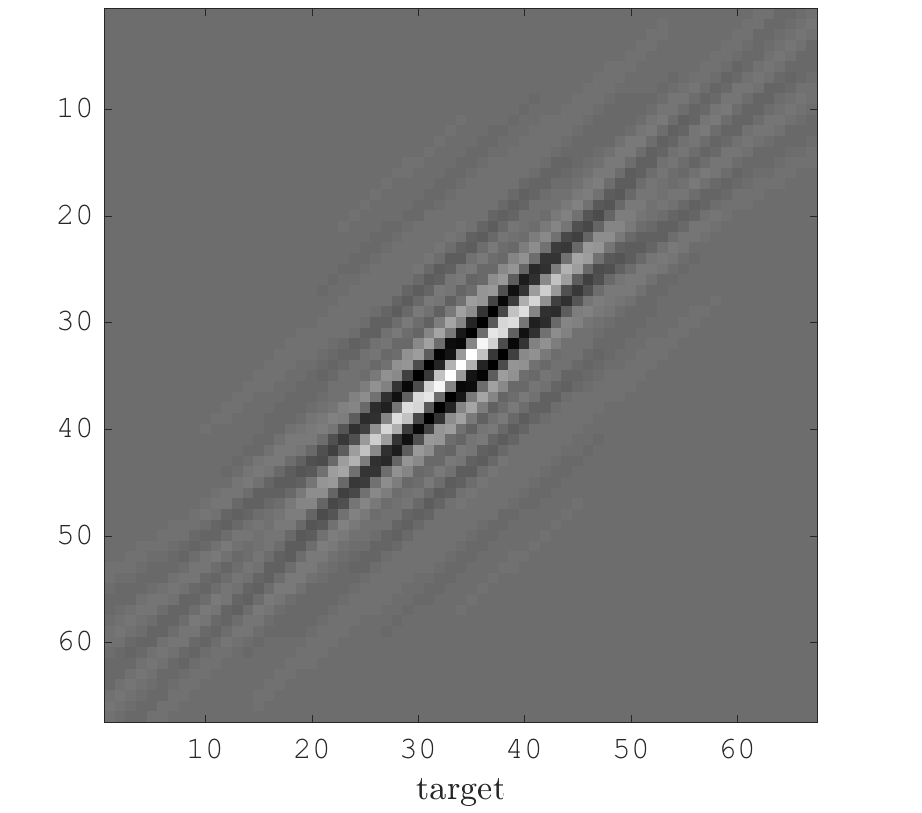
\includegraphics[width=\textwidth]{figures/xp/xp_128x128_sc2_angl1_K3_S3_node1_target.png}
    \end{subfigure}
\begin{subfigure}[b]{0.49\textwidth}\centering
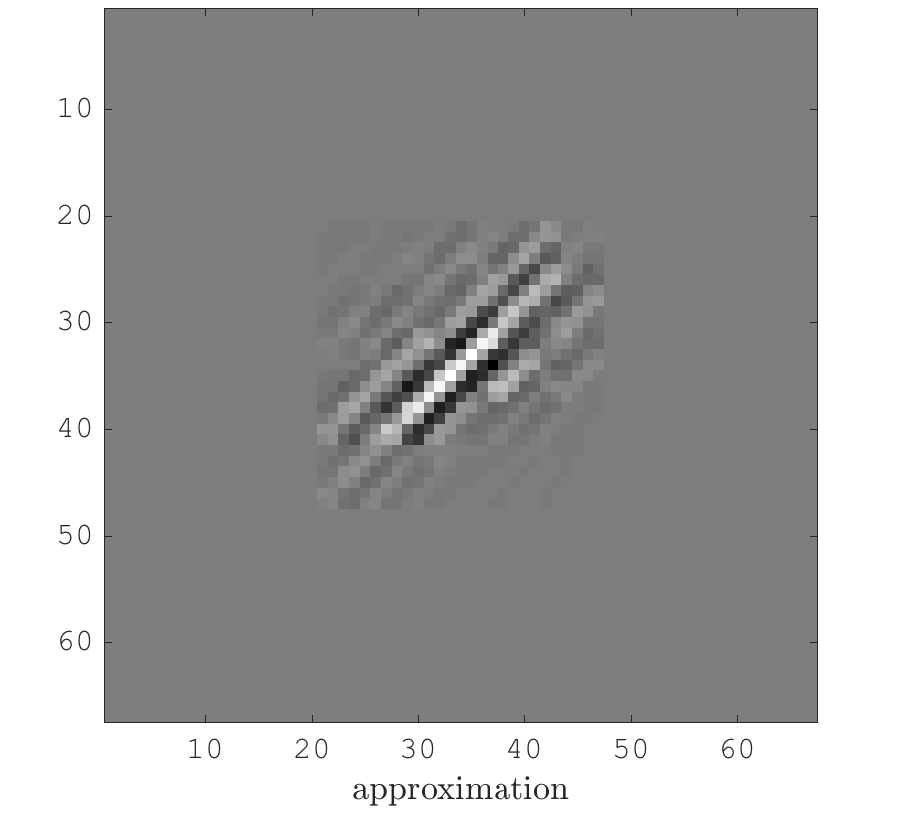
\includegraphics[width=\textwidth]{figures/xp/xp_128x128_sc2_angl1_K3_S3_node1_approx.png}
\end{subfigure}
    \begin{subfigure}[b]{0.49\textwidth}\centering
    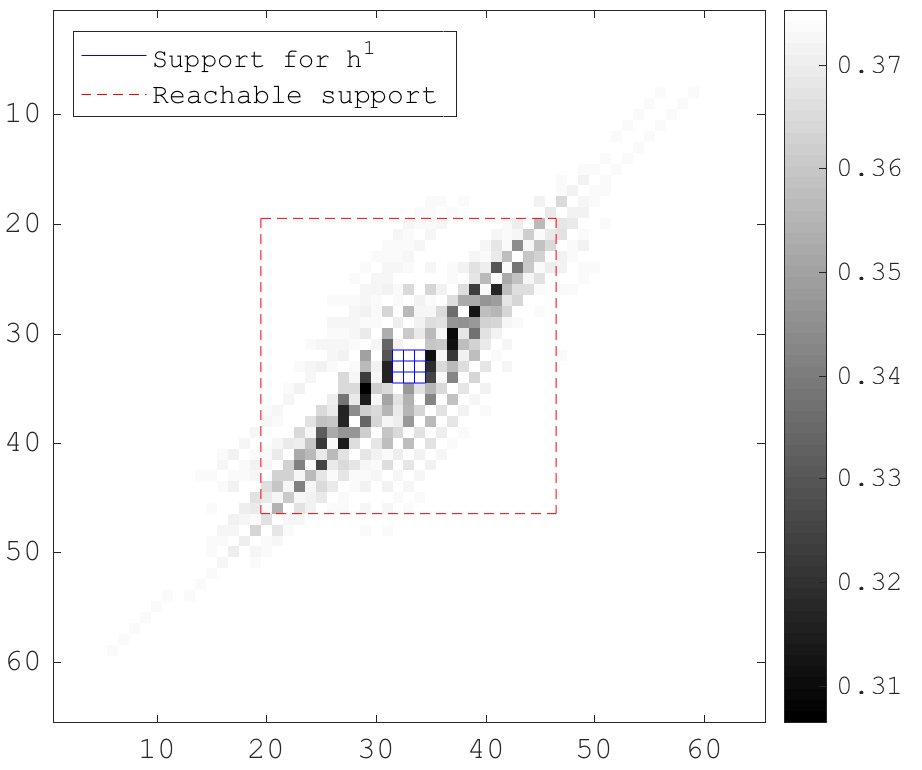
\includegraphics[width=\textwidth]{figures/xp/xp_128x128_sc2_angl1_K3_S3_node1_obj_matrix.png}
    \end{subfigure}
    \begin{subfigure}[b]{0.49\textwidth}\centering
    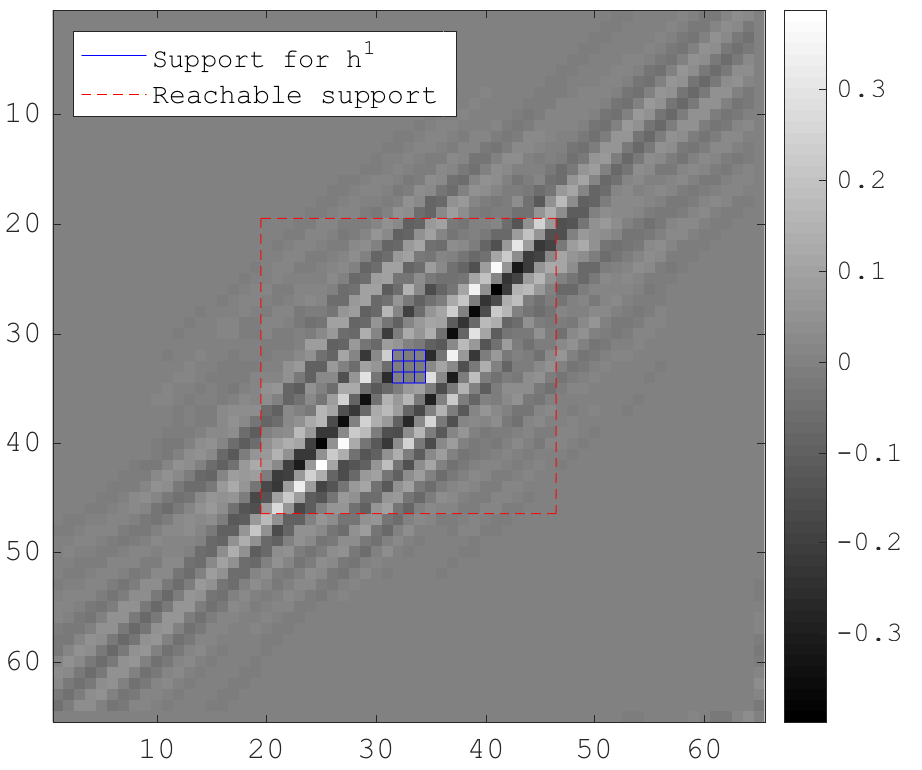
\includegraphics[width=\textwidth]{figures/xp/xp_128x128_sc2_angl1_K3_S3_node1_gradient_node_1.png}
    \end{subfigure}
\end{figure}

\begin{table}[!h]\centering
\begin{tabular}{@{}lll@{}}\toprule
 & RMSE & Relative RMSE \\ \midrule
Before & 0.004786 & 0\% \\
After & 0.004325 & 9.6\% \\ \bottomrule
\end{tabular}
\caption{RMSE comparison when adding to the support on the \nth{1} edge. Note that for the "added point" RMSE, we took the minimum of all RMSE for every point possibly added. Here, the RMSE is at best increased by 9.6\%.}
\end{table}


\begin{figure}[!h]\centering
    \begin{subfigure}[b]{0.49\textwidth}\centering
    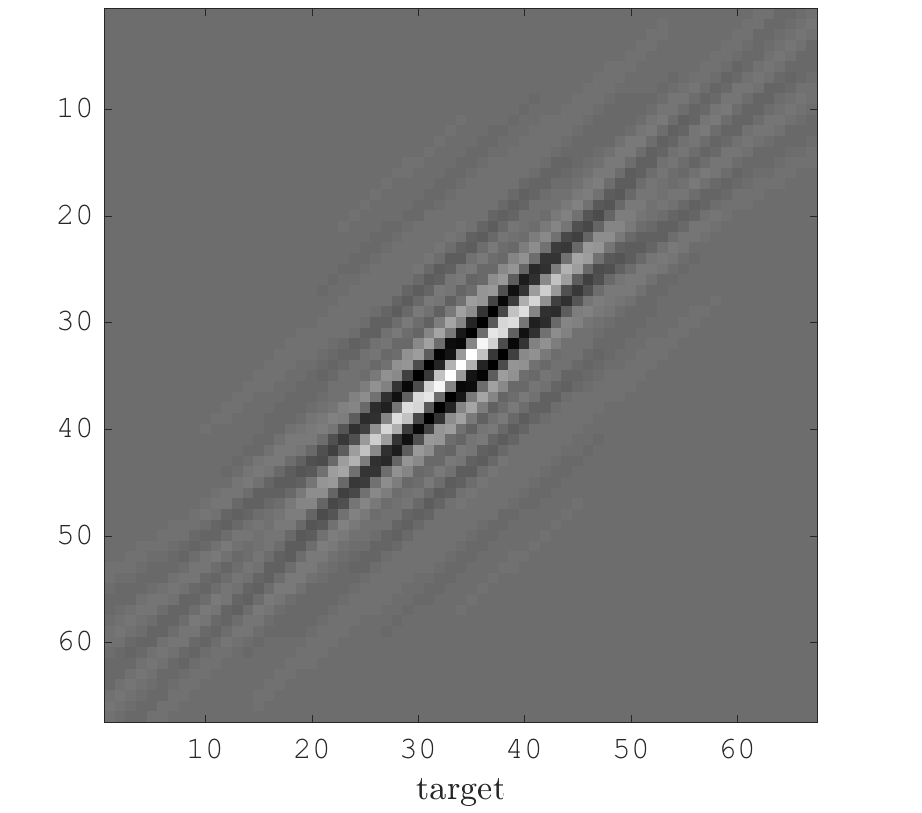
\includegraphics[width=\textwidth]{figures/xp/xp_128x128_sc2_angl1_K3_S3_node2_target.png}
    \end{subfigure}
\begin{subfigure}[b]{0.49\textwidth}\centering
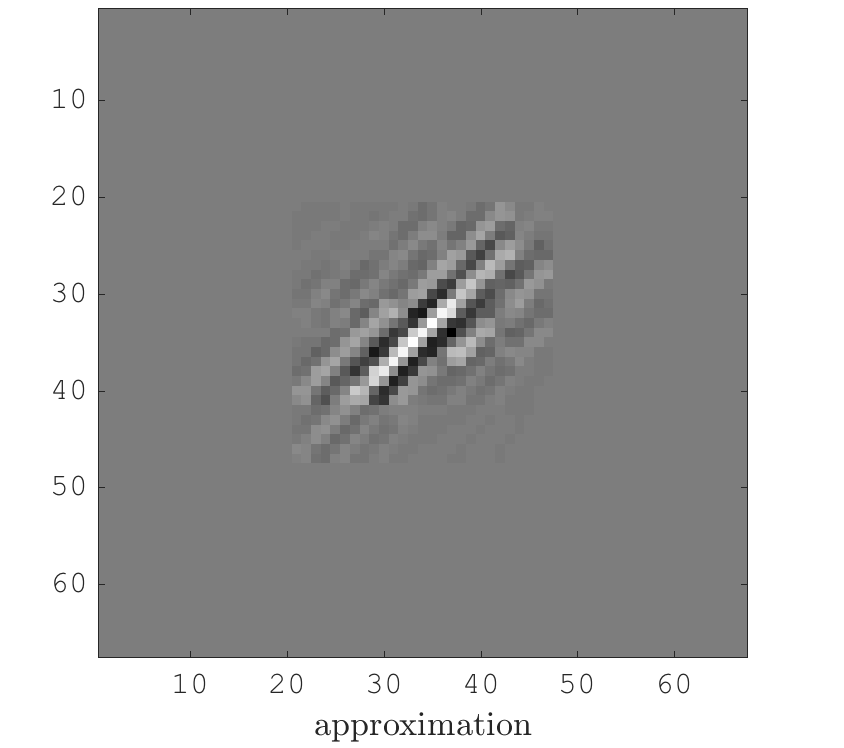
\includegraphics[width=\textwidth]{figures/xp/xp_128x128_sc2_angl1_K3_S3_node2_approx.png}
\end{subfigure}
   \begin{subfigure}[b]{0.49\textwidth}\centering
    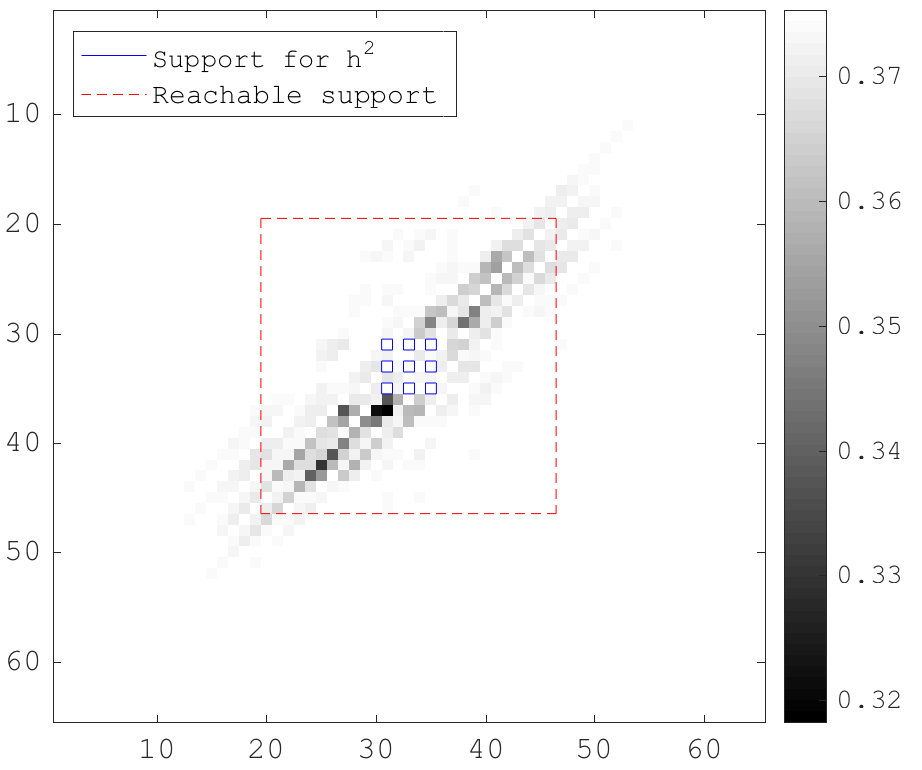
\includegraphics[width=\textwidth]{figures/xp/xp_128x128_sc2_angl1_K3_S3_node2_obj_matrix.png}
    \end{subfigure}
    \begin{subfigure}[b]{0.49\textwidth}\centering
    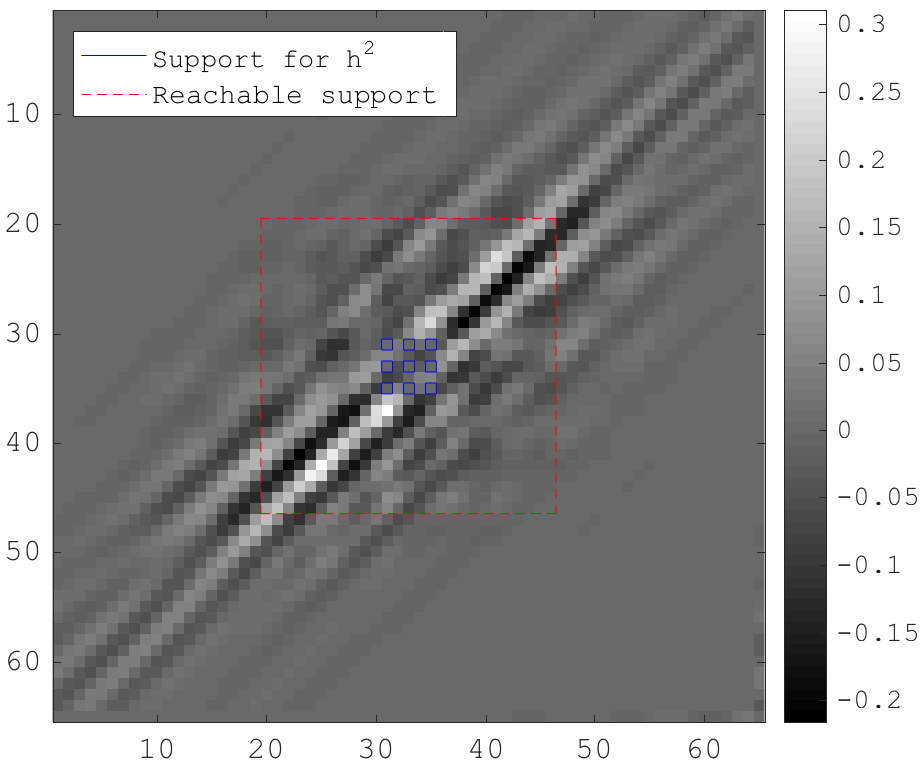
\includegraphics[width=\textwidth]{figures/xp/xp_128x128_sc2_angl1_K3_S3_node2_gradient_node_2.png}
    \end{subfigure}
\end{figure}

\begin{table}[!h]\centering
\begin{tabular}{@{}lll@{}}\toprule
 & RMSE & Relative RMSE \\ \midrule
Before & 0.004786 & 0\% \\
After & 0.004407 & 7.9\% \\ \bottomrule
\end{tabular}
\caption{RMSE comparison when adding to the support on the \nth{2} edge}
\end{table}


\begin{figure}[!h]\centering
    \begin{subfigure}[b]{0.49\textwidth}\centering
    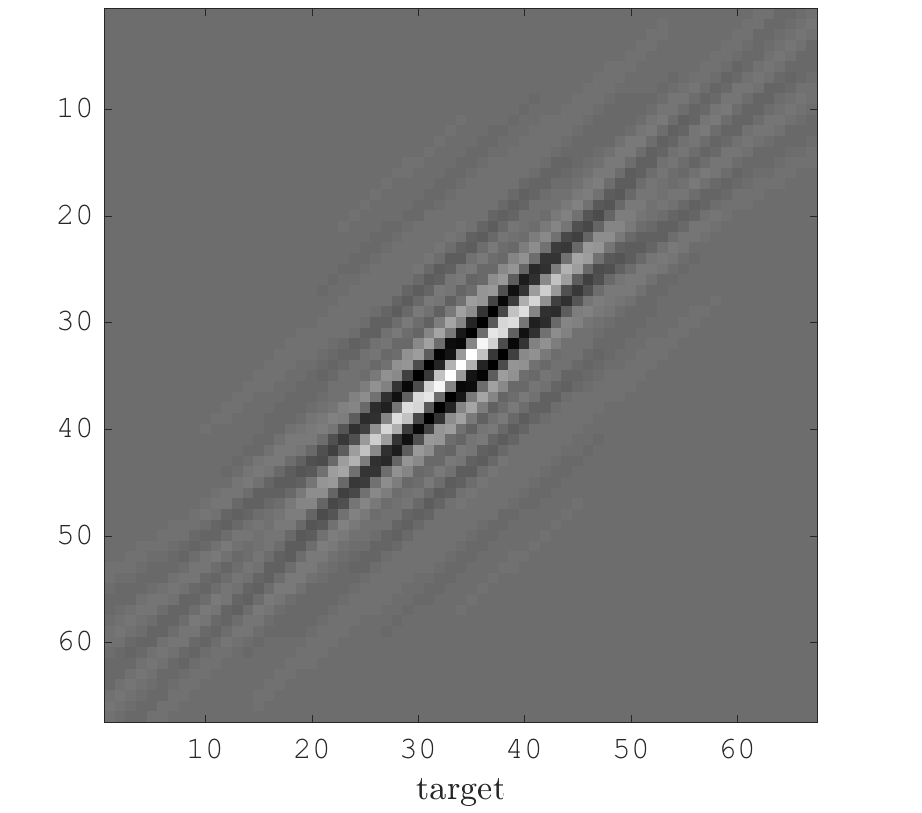
\includegraphics[width=\textwidth]{figures/xp/xp_128x128_sc2_angl1_K3_S3_node3_target.png}
    \end{subfigure}
\begin{subfigure}[b]{0.49\textwidth}\centering
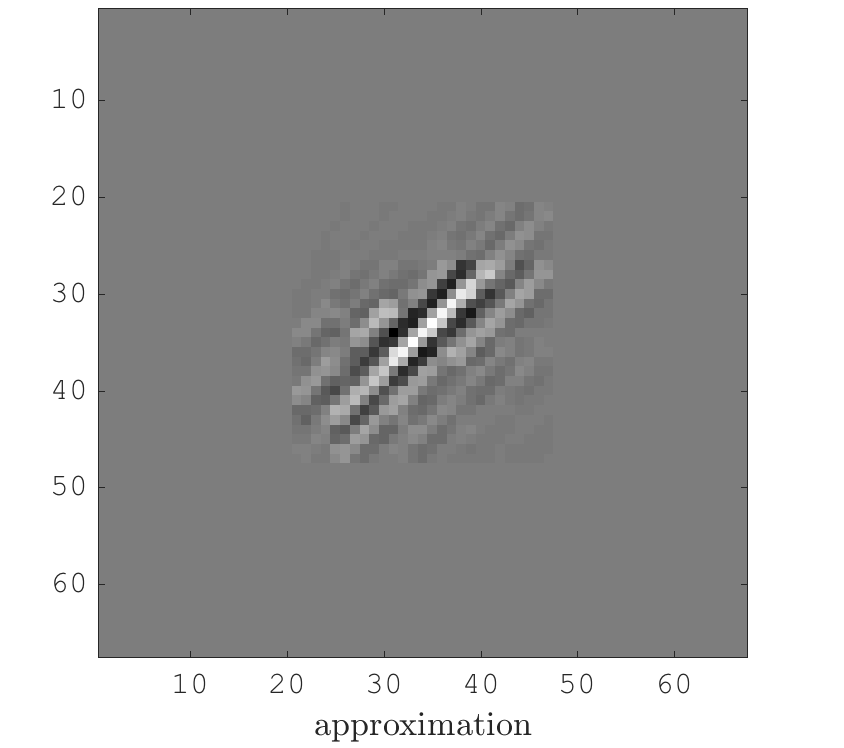
\includegraphics[width=\textwidth]{figures/xp/xp_128x128_sc2_angl1_K3_S3_node3_approx.png}
\end{subfigure}
   \begin{subfigure}[b]{0.49\textwidth}\centering
    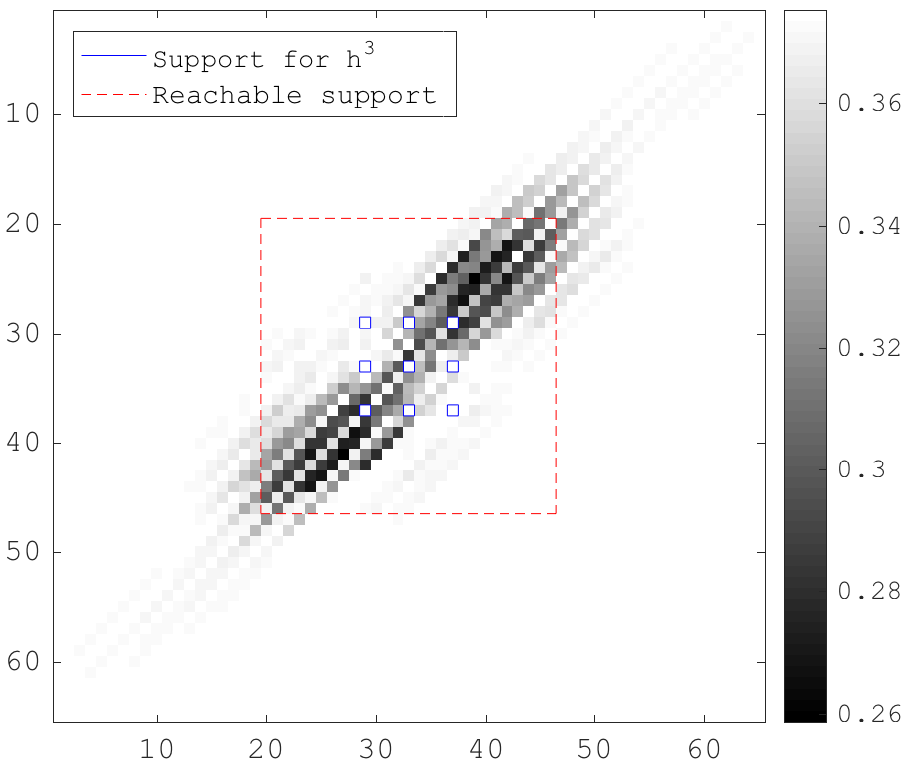
\includegraphics[width=\textwidth]{figures/xp/xp_128x128_sc2_angl1_K3_S3_node3_obj_matrix.png}
    \end{subfigure}
    \begin{subfigure}[b]{0.49\textwidth}\centering
    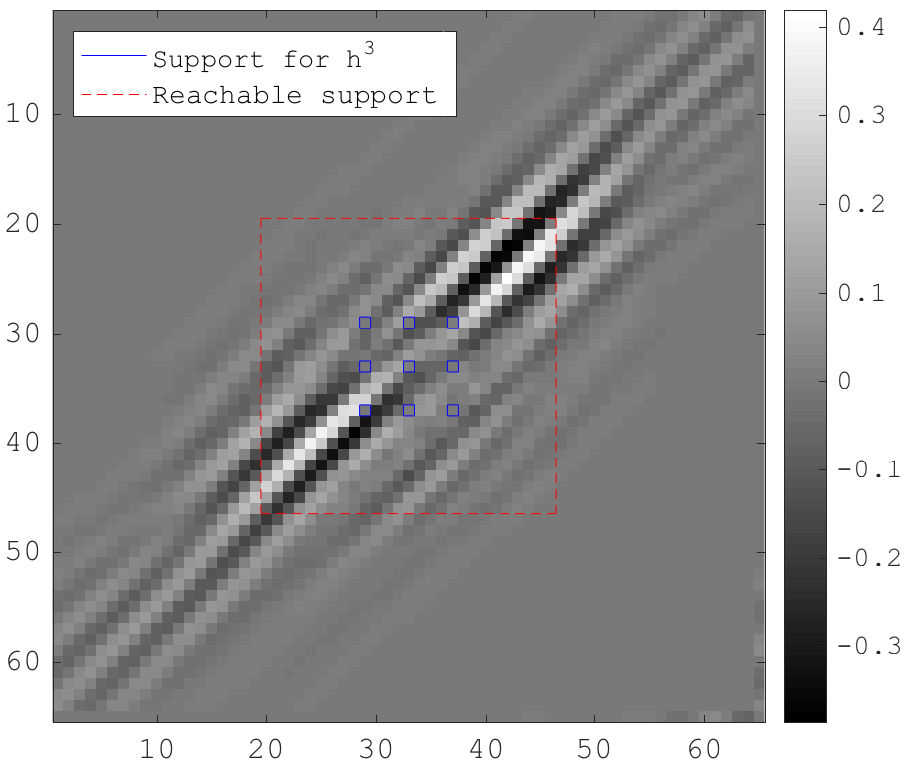
\includegraphics[width=\textwidth]{figures/xp/xp_128x128_sc2_angl1_K3_S3_node3_gradient_node_3.png}
    \end{subfigure}
\end{figure}


\begin{table}[!h]\centering
\begin{tabular}{@{}lll@{}}\toprule
 & RMSE & Relative RMSE \\ \midrule
Before & 0.004786 & 0\% \\
After & 0.003973 & 16.9\% \\ \bottomrule
\end{tabular}
\caption{RMSE comparison when adding to the support on the \nth{3} edge}
\end{table}


\begin{figure}[!h]\centering
    \begin{subfigure}[b]{0.49\textwidth}\centering
    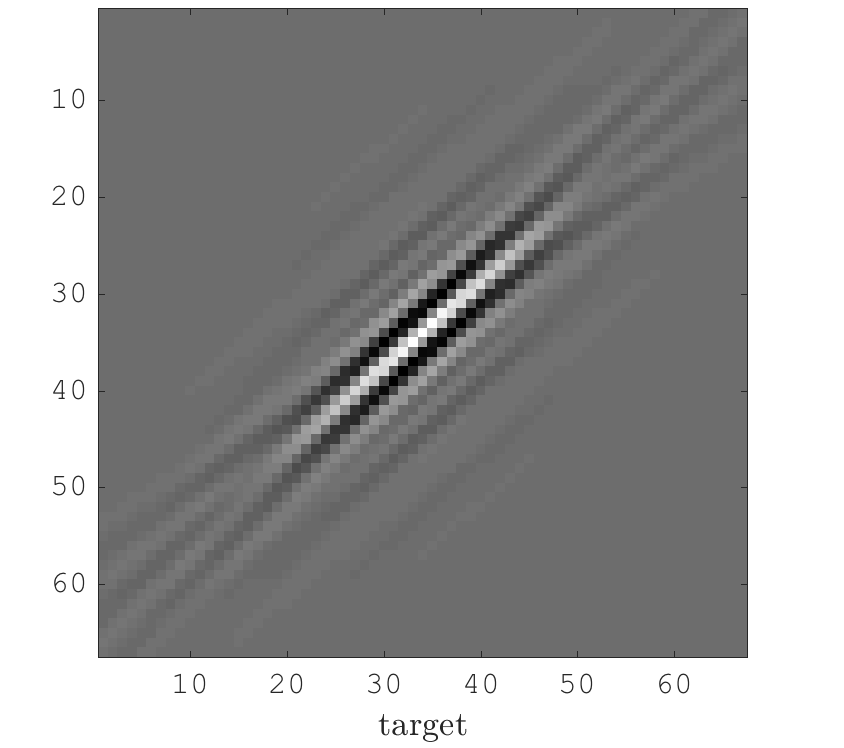
\includegraphics[width=\textwidth]{figures/xp/xp_128x128_sc2_angl1_K3_S3_node4_target.png}
    \end{subfigure}
\begin{subfigure}[b]{0.49\textwidth}\centering
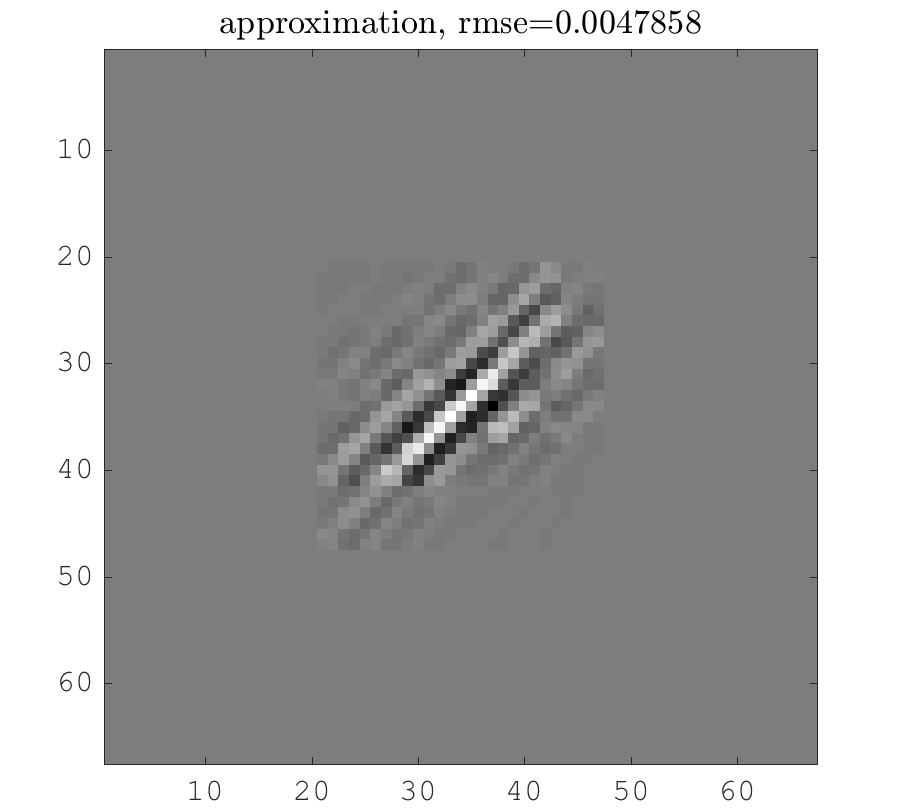
\includegraphics[width=\textwidth]{figures/xp/xp_128x128_sc2_angl1_K3_S3_node4_approx.png}
\end{subfigure}
   \begin{subfigure}[b]{0.49\textwidth}\centering
    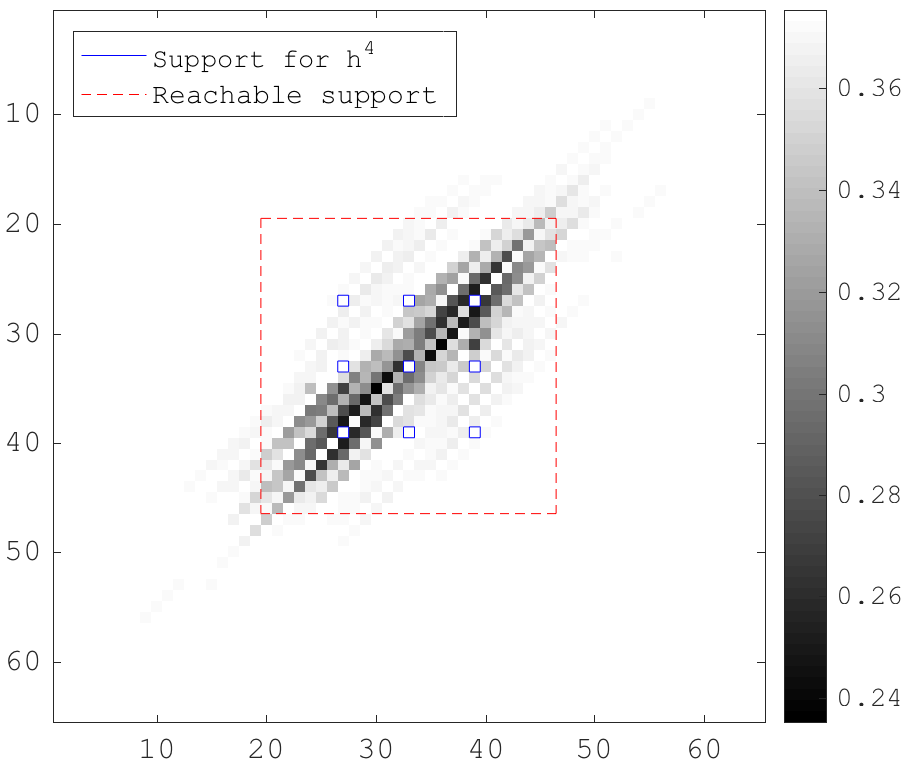
\includegraphics[width=\textwidth]{figures/xp/xp_128x128_sc2_angl1_K3_S3_node4_obj_matrix.png}
    \end{subfigure}
       \begin{subfigure}[b]{0.49\textwidth}\centering
    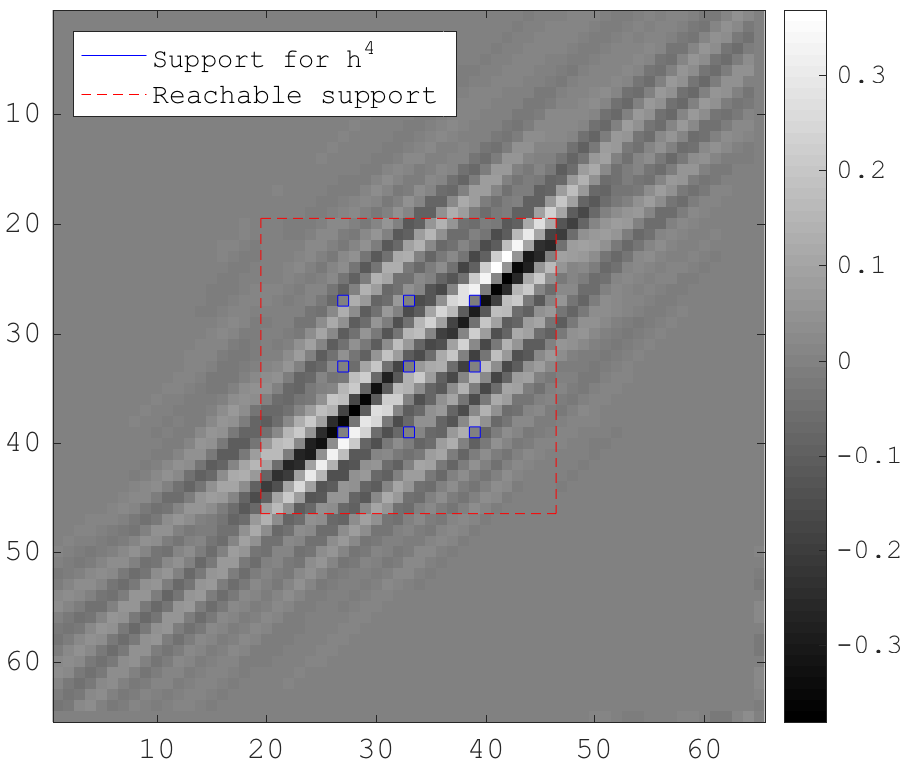
\includegraphics[width=\textwidth]{figures/xp/xp_128x128_sc2_angl1_K3_S3_node4_gradient_node_4.png}
    \end{subfigure}
\end{figure}

\begin{table}[!h]\centering
\begin{tabular}{@{}lll@{}}\toprule
 & RMSE & Relative RMSE \\ \midrule
Before & 0.004786 & 0\% \\
After & 0.003790 & 20.8\% \\ \bottomrule
\end{tabular}
\caption{RMSE comparison when adding to the support on the \nth{4} edge}
\end{table}

% XXX Proof not finished; this proof might be useless/overkill in my thesis...
\begin{align*}
(\widehat{\widetilde{A}})_{m,n} =& \sum_{k=1}^M \sum_{l=1}^N \widehat{A}_{k,l} e^{-2i\pi (k\frac{m}{M}+l \frac{n}{N})}\\
=& \sum_{k=1}^M \sum_{l=1}^N A_{-k,-l} e^{-2i\pi (k\frac{m}{M}+l \frac{n}{N})}\\
\shortintertext{By changing variables $k'=-k$ and $l'=-l$, we get:}
=& \sum_{k'=-M}^{-1} \sum_{l'=-N}^{-1} A_{k',l'} e^{2i\pi (k'\frac{m}{M}+l' \frac{n}{N})}
\shortintertext{And thanks to the $(M,N)$ periodicity of $A$, which means that $A_{i,j}=A_{i+kM,j+lN}$, $\forall (k,l) \in \mathbb{N}^2$, letting us with:}
=& \sum_{k'=-M}^{-1} \sum_{l'=-N}^{-1} A_{k'+M,l'+N} e^{2i\pi (k'\frac{m}{M}+l' \frac{n}{N})}\\
\shortintertext{With a second change of variables $k''=k'+M$ and $l''=l'+N$:}
=& \sum_{k''=-M+M}^{-1+M} \sum_{l''=-N+N}^{-1+N} A_{k'',l''} e^{2i\pi (k'\frac{m}{M}+l' \frac{n}{N})}\\
=& \sum_{k'=1}^{M} \sum_{l'=1}^{N} A_{k',l'} e^{2i\pi (k'\frac{m}{M}+l' \frac{n}{N})}
\end{align*}


%---------- USELESS \\
Note: I first wrote it using indices running from 1 to N, but it creates a kind of "glitch" that breaks the symmetry... With a signal $x$ that spans in $[1;3]$. As this signal is periodical, you get the same values at $[1+3;3+3]=[4;6]$. The generalization gives $x_i = x_{i+kN}$ with $k\in\mathbb{N}$. But starting at 1 prevents from generalizing to negative $k$.
\begin{table}\centering\begin{tabular}{lllllllllll}\hline 
-3 & -2 & -1 & \multicolumn{1}{l|}{0} & 1 & 2 & \multicolumn{1}{l|}{3} & 4 & 5 & \multicolumn{1}{l|}{6} & 7 \\ \hline
\multicolumn{4}{c}{Signal?} & \multicolumn{3}{c}{Signal} & \multicolumn{3}{c}{Signal} & 
\end{tabular}\end{table}
Indeed, $[1-3;3-3]=[2;0]$
% ------------------------ \\
\end{document}



